\chapter{Математический аппарат для моделирования}

\section{Метод конечных разностей}
Суть метода конечных разностей заключается в аппроксимации дифференциальных операторов отношением конечных разностей. Так например производную некоторой функции $y(x)$ в точке $x_{0}$ ($\dot{y}(x_{0})$) можно представить \cite{Samarski}:
\begin{gather}
	\dot{y}_{+}(x_{0}) = \frac{d}{dx}y(x_{0}) = \frac{y(x_{0} + \Delta x) - y(x_{0})}{\Delta x };\\
	\dot{y}_{-}(x_{0}) = \frac{d}{dx}y(x_{0}) = \frac{ y(x_{0}) - y(x_{0} - \Delta x)}{\Delta x };\\
	\dot{y}_{-}(x_{0}) = \dot{y}_{+}(x_{0}) = \frac{d}{dx}y(x_{0}),
\end{gather}
\begin{conditions}
	$\dot{y}_{-}$ & производная слева;\\
	$\dot{y}_{+}$ & производная справа;\\
	$\Delta x$ & приращение аргумента (шаг сетки).
\end{conditions}

$\Delta x$ -- это шаг нашей конечно-разностной схемы (аппроксимации). Если шаг сетки постоянен, то говорят о регулярной сетке, иначе о нерегулярной. Мы будем рассматривать только регулярные сетки. Далее вместо $\Delta x$ будет использовать $\Delta$.

Из выше сказанного можно найти трехточечную аппроксимацию второй производной $y(x)$:
\begin{gather}
	\label{eq:3dots}
	\frac{d^{2}}{dx^{2}}y(x_{0}) = \frac{\dot{y}_{+} - \dot{y}_{-}}{\Delta} = \frac{y(x_{0} + \Delta) - 2y(x_{0}) + y(x_{0} - \Delta)}{ \Delta^{2}}.
\end{gather}

Для связи конечно-разностной схемы по времени и координате для нестационарного уравнения диффузии (\ref{eq:F2}) воспользуемся апроксимацией двухточечной апроксимацией первой производной и по времени и трехточечной апроксимацие второй производной по координате: 
\begin{equation}
	\label{eq:xt}
	\frac{C^{j+1}_{i} - C^{j}_{i}}{\Delta t} = \frac{C^{j}_{i-1} - 2C^{j}_{i} + C^{j}_{i+1}}{ \Delta^{2}},
\end{equation}

\begin{conditions}
	$C^{j}_{i}$ & значение функции в точке $i$, в момент времени $j$;\\
	$\Delta t$ & шаг сетки по времени;\\
	$\Delta x$ & шаг сетки по координате.
\end{conditions}

Трехточечную апроксимацию производной (конечно-разностную схему) (\ref{eq:3dots}) можно наглядно показать, как:
\begin{figure}[h!]
	\centering
	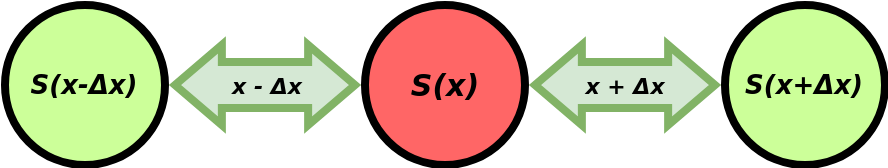
\includegraphics[width=\linewidth]{assets/Approx}
	\caption{Графическая схема для конечно-разностной схемы (\ref{eq:3dots})}
	\label{fig:3dots}
\end{figure}\\
\begin{conditions}
	$S(x)$ & состояние системы в точке $x$;\\
	$\Delta x$ & шаг сетки (приращение аргумента).
\end{conditions}

Конечно разностную схему (\ref{eq:xt}) наглядно можно представить так:
\begin{figure}[h!]
	\centering
	\includegraphics[width=\linewidth]{assets/Diffusion}
	\caption{Графическая схема для конечно-разностной схемы (\ref{eq:xt})}
	\label{fig:xt}
\end{figure}\\
\begin{conditions}
	$S(x, t)$ & состояние системы в момент $t$ и точке $x$;\\
	$\Delta x$ & приращение по координате;\\
	$\Delta t$ & приращение по времени.
\end{conditions}
